% Copyright (C) 2022 Haoqing Xu
% School of Artificial Intelligence, Southeast University.
% --------------------------------------------------------------------------

% This work may be distributed and/or modified under the
% conditions of the LaTeX Project Public License, either
% version 1.3c of this license or (at your option) any later
% version. This version of this license is in
%    http://www.latex-project.org/lppl/lppl-1-3c.txt
% and the latest version of this license is in
%    http://www.latex-project.org/lppl.txt
% and version 1.3 or later is part of all distributions of
% LaTeX version 2005/12/01 or later.

% This work has the LPPL maintenance status `maintained'.
% The Current Maintainer of this work is Haoqing Xu.

% Home Page of the Project: https://github.com/SuikaXhq/seu-bachelor-thesis-2022
\documentclass{seuthesis-2022}


\title{}
\titlea{}
\titleb{}
\author{}
\studentnum{}
\department{}
\major{}
\supervisor{}
\date{}

\begin{document}

\maketitle

\makedeclaration

\begin{abstract}[zh]
    
\end{abstract}

\begin{abstract}[en]
    
\end{abstract}

\tableofcontents

\section{绪论}
\subsection{课题背景和意义}
绪论部分主要论述选题的意义、国内外研究现状以及本文主要研究的内容、研究思路以及内容安排等。

章标题为三号黑体加粗居中;一级节标题(如,2.1 本文研究内容):四号黑体居左;二级节标题(如,2.1.1 实验方法):小四号宋体居左。

正文部分为小四号宋体,行间距1.5倍行距,首行缩进2个字符。

\subsection{研究现状}

\subsection{本文研究内容}

\subsection{正文}
正文部分每一章应另起页书写书写,层次要清楚,内容要有逻辑性,正文一般不少于15000字。正文部分因学科、选题特点可有差异,但必须言之成理,论据可靠,严格遵循本学科国际通行的学术规范。

中文为小四号宋体,英文及数字为小四号Times New Roman,首行缩进2个字符,行间距为1.5倍。

\subsection{插图格式要求}
插图力求精炼,且每个插图均应有图序和图名。图序与图名位于插图下方,图序一般按章节编排,如图1-1(第一章第1个图),在插图较少时可以全文连续编序,如图10。

如一个插图由两个及以上的分图组成,分图用(a)、(b)、(c)等标出,并标出分图名。

简单文字图可用WORD直接绘制,复杂的图考虑使用相应的图形绘制软件完成,以提高图形表达质量。

插图居中排列,与上文文本之间空一行。图序图名设置为五号宋体居中,图序与图名之间空一格。

\begin{figure}[H]
    \centering
    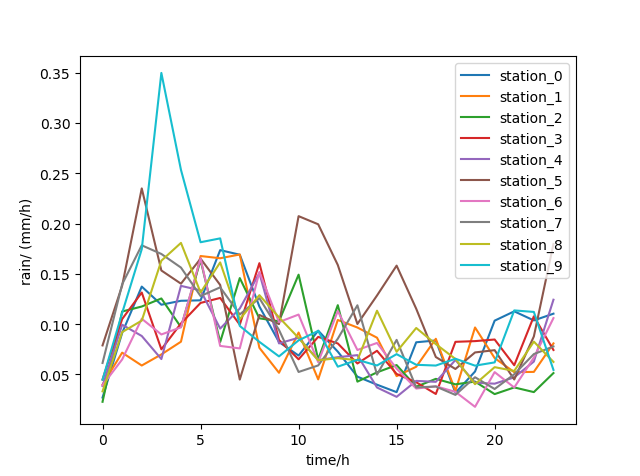
\includegraphics{fig/降水量均值分布图.png}
    \caption{每小时降水量24小时均值分布图}
    % \label{fig:my_label}
\end{figure}

\begin{figure}[H]
    \centering
    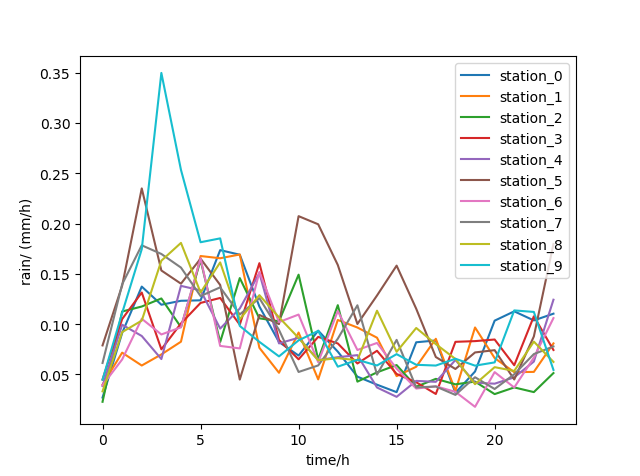
\includegraphics{fig/降水量均值分布图.png}
    \caption{每小时降水量24小时均值分布图}
    % \label{fig:my_label}
\end{figure}

\end{document}